\chapter{Introduction}
\label{ch:intro}
\startchapter

%\isec{Setting the stage}

Elite sport coaches are always looking for new insights into their team's performance.

The rise of \textit{Sabermetrics}\footnote{Phil Birnbaum, ``A Guide to Sabermetric Research'', Society for American Baseball Research. \url{https://sabr.org/sabermetrics}} in baseball, originally developed in the 1970's and later popularised in the book and film \textit{Moneyball} \cite{Lewis2004}, is evidence of a historic shift of coaching attitudes. Reliance on coaching hunches and intuition to select and train players has been largely overthrown in favour of data driven decision making approaches based on quantitative performance metrics.\footnote{Leigh Steinberg, 18 Aug 2015, ``Changing the Game: The Rise of Sports Analytics'', Forbes. \url{https://www.forbes.com/sites/leighsteinberg/2015/08/18/changing-the-game-the-rise-of-sports-analytics/}}

Traditionally, data driven approaches to sport analysis have been limited to simple mathematical formulas based on manually observable attributes, such as the number of runs made by each player in cricket, or the number of possessions by each player in basketball. However, with the rise of low cost position tracking devices, such as computer vision tracking systems and self-contained GPS tracking units, there has been an explosion in the depth of data available\footnote{The technological advances that have resulted in rich datasets will be discussed at length in \secref{literature-review}.} which creates opportunities for new approaches to sport analysis.

Currently, these tracking devices are being used by sport performance analysts to analyse individual players. They are used to answer questions such as: \textit{How far did the player run?} \textit{What was their maximum speed?} \textit{Considering the player's past movement intensities and durations, at what point should the player be interchanged to prevent fatigue or injury?}

However, teamwork is about more than a group of individual players.\footnote{Matti Clements, ``How to get your group to become a team'', \textit{Sports Coach}, Australian Sports Commission. %, vol. 29 no. 2.
\url{https://web.archive.org/web/20151102065854/http://www.ausport.gov.au/sportscoachmag/psychology2/how_to_get_your_group_to_become_a_team}} As the devices allow tracking every member of the team, they offer the potential to quantify the team dynamics as a whole. They could be used to answer questions such as: \textit{Which formations lead to goals?} \textit{How do these formations change over time?} \textit{Are any players out of formation?} \cite{LeHoang2017}

%\isec{Background to introduce spatio-temporal analysis. i.e. importance of both space \textit{and} time together}

\section{Spatio-Temporal Analysis}

% Introduce spatio-temporal analysis.
A crucial domain concern for sport strategy, particularly in \textit{team invasion games} such as Association Football (soccer), basketball, and Australian Rules Football, is the control of space on the field over time \cite{Coventry2015}. There are mature systems for spatial analysis, such as Geographic Information Systems (\gls{gis}), as well as for time series analysis. However as space and time are intricately interlinked, seamlessly integrating spatial and temporal analysis as a unified system remains a challenge; areas such as the design of \textit{Moving Object Databases} \cite{schneider2009moving} and design of appropriate visualisation techniques for large scale trajectory data \cite{andrienko_visualization_2014} are still an active area of research. The set of analysis methods at the intersection of spatial and temporal analysis are referred to as \textit{spatio-temporal} analysis methods. The application of suitable spatio-temporal analysis methods to the context of sport is the key to extracting insights that can more fully utilise the high-dimensional data generated by position tracking sensors.

%\isec{Motivation / Problem}

The objective of this thesis is to bring spatio-temporal analysis techniques within reach for sport researchers and practitioners so as to facilitate their widespread adoption for analysis of games. Statistical platforms such as \textit{R} contain a large library of existing spatio-temporal algorithms and techniques which are freely available. However, pre-existing spatio-temporal analysis algorithms cannot be meaningfully applied to sport position tracking as-is without first transforming the data into an amenable form. For example, movements during the half-time break need to be discarded, and the field orientation and goal directions need to be accounted for such that the direction of attacking goals is in a consistent direction for each data point. Attempting to apply an existing spatial analysis algorithm without first accounting for this would lead to a meaningless result. As such, a major portion of this thesis is dedicated to building a solid foundation for transforming raw sport position tracking data into an form that sport practitioners can utilise, such as \figref{fig:introsample}. %and enables further analysis.

\begin{figure}[!htb]
\centering
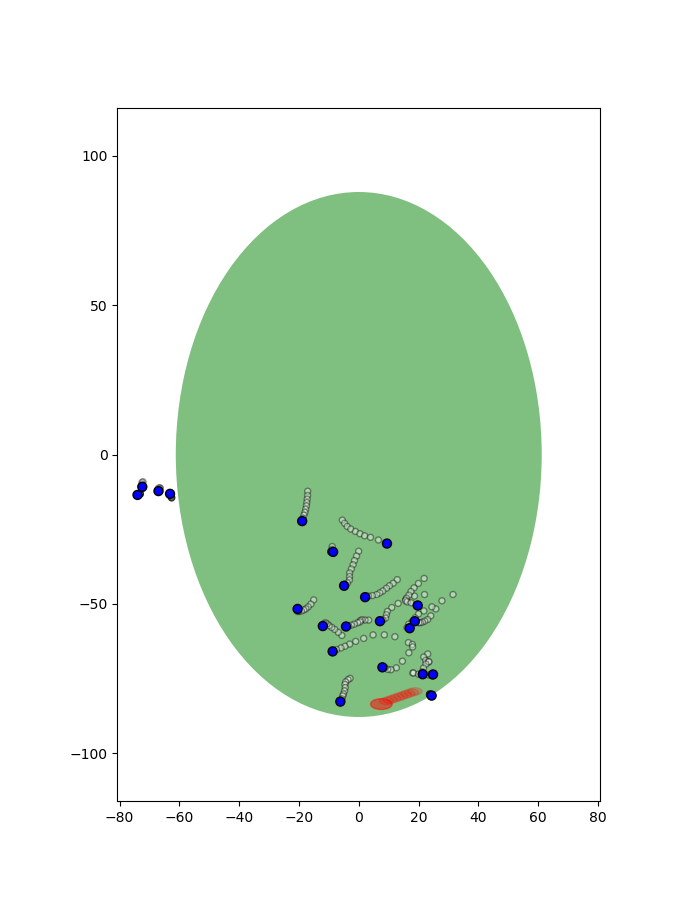
\includegraphics[width=0.6\linewidth]{ds-r9-q1-frames-combo-frame000204.png}
\caption{Visualisation of team GPS tracking data. The blue dots represent the position of the team. The red oval represents the position of the ball. The trails represent past movements. The group of four players on the left are the interchange/substitute players. Creating this visualisation requires preprocessing steps to reproject the latitudes and longitudes reported by the GPS tracking devices into the coordinate system of the field and to synchronise with the ball tracking data. This forms the foundation for further quantitative investigation of team formations.
\label{fig:introsample}}
\end{figure}

\section{Computational Pipelines}

Conducting sport research requires a \textit{workflow} of operations such as player de-identification, data selection, data normalisation, visualisation, and statistical analysis. In contrast to computation of traditional sport statistics, the additional scope for data exploration permitted by spatio-temporal data sources can lead to complex workflows that become difficult for humans to manage. Even if each operation in the workflow is an automated computer program, remembering which inputs and outputs to feed to each operation and how they connect together can become unmanageable as the workflow grows to integrate additional data sources and analysis outputs. A \textit{pipeline} is a sequence of such operations chained together to automate the entire workflow end-to-end.

%\isec{Introduction to computational pipelines}

Advances in data collection and processing have made highly sophisticated data analysis workflows feasible to facilitate greater depth of data analysis. However, unless the demand for increasingly sophisticated analysis workflows coincides with development of appropriate tools to manage this complexity, there is a risk that the rigour will suffer as a result of others being unable to reliably repeat the process. \textit{Nature} has reported growing evidence of a ``reproducibility crisis'' \cite{Baker2016} wherein scientists in every discipline have admitted to being unable to reproduce other's experiments, or even their own work. Scientific fields that deal with analysis of large volumes of data, such as bioinformatics, have recognised the need for development of automated \textit{computational pipelines} \cite{Goodstadt2010} and \textit{workflow managment systems} \cite{Oinn2004, Hull2006} to help ensure that the analysis process is repeatable.

Tools originally developed to allow creation of complex bioinformatics pipelines (e.g. analysis of DNA sequences) include Apache Taverna \cite{Oinn2004, Hull2006} and Python Ruffus \cite{Goodstadt2010}. In principle, these tools can also be used as general frameworks for data processing and analysis in other domains such as sport. However, it is well known amongst designers of Domain Specific Languages (DSLs) that generality and flexibility run counter to the needs of supporting concise expression of a particular domain \cite{Voelter2013}. Thus, while a range of domain specific and general frameworks for constructing pipelines exist, new frameworks and components are needed to build a software ecosystem for spatio-temporal analysis in the sport domain.

Being able to reproduce the end result of a process is not enough---auditing complex processes to validate and debug them requires a record of \textit{data provenance} (i.e. the ability to trace the flow of data, particularly at the boundaries of sub-systems). Data provenance gives analysts the ability to trace the flow of data backward so they can answer questions about the data sources and specific data records that were used to calculate the results of an analysis. For example, if a sport practitioner arrives at an unexpected result, a player or coach may request to see the underlying video sequences for events in the game that contributed to that result.

% This is particularly important to sport practitioners, as sport practitioners need to be able to translate the findings back to game scenarios. For example, if a sport practitioner arrives at an unexpected result, a player or coach may request to see the video sequences for events in the game that contributed to that result.

%\isec{Value of studying data transformations in the context of sport rather than reusing a general solution from another field}

Common data operations required for spatial analysis of sport include: de-identifying players; normalising spatial data with respect to the playing field; mining spatio-temporal patterns; and aggregating and visualising the results. Each of these is a form of \textit{data transformation}. Each transformation is introduced below, and an explanation is given of how the transformation is interwoven with the concerns of the sport domain:

\textbf{De-identifying players}\hs While it is trivial to partially de-identify sensitive player data by replacing player names with unique codes, ensuring that the data are truly non-identifiable requires consideration of all possible linkages to other sport datasets that could be used to re-identify a player. Specifically, when de-identified players are associated with movement data, there is a high risk that the player could be re-identified through fingerprinting techniques that correlate game events detected in the movement data (such as kicks, tackles or interchanges) with public match feeds and televised match video footage that contain the player name alongside the actions they performed.\footnote{The importance of properly de-identifying sport data to protect player privacy, and the unique challenges to the de-identification process posed by player tracking data are discussed in detail within \chref{ch:de-identification}.}

\textbf{Normalising spatial data}\hs When dealing with spatio-temporal datasets where local movements are more important than global movements, one should consider normalising the data with respect to a reference frame. In sport, there is a need to normalise with respect to the playing field. Specific types of sport may have additional requirements that affect how the normalisation is performed. For example, in Australian Rules Football, each field has a different size, shape, and orientation that need to be accounted for.

\textbf{Aggregating data}\hs Realising the promised potential of automated team-level spatio-temporal analysis requires a sufficient number of scoring formations to detect subtle patterns in a statistically sound manner. Even in Australian Rules Football---which is considered a fast paced sport---each team scores only 25 times\footnote{Average number of scoring events derived from 1897-2018 match data from \url{afltables.com}, retrieved 2018-05-21} (on average) over the course of any given match. Thus it is necessary to aggregate data from many different sport fields into a large unified dataset that can be mined for patterns.

\textbf{Mining spatio-temporal patterns}\hs In sport, the spatial movements of players are related to the ``phase'' of the game (e.g. defence/offence). Thus spatio-temporal analysis cannot be conducted in isolation; detected patterns need to be analysed within the context of transitions between phases of play.

\textbf{Visualising results}\hs Visualisation is also a form of data transformation \cite{Jankun-Kelly2007}. Visualisations need to consider the domain in order to optimally map data attributes to visual attributes \cite{Moody2009}. Specifically, visualisations are needed for presenting de-identified Australian Rules Football player position tracking data in a form interpretable by sport practitioners that permits exploration and comparisons of different matches.

While the transformations described above may at first appear to be common data operations available in existing data analysis software, generalised approaches fail to adequately address the specific needs of sport analysis and thus suffer from the ``leaky abstraction''\footnote{In software engineering, ``abstraction'' refers to the process of generalising concepts to allow them to be used at a high-level without the need to concern oneself with all the low-level implementation details (for example, one may abstract away the details of how GPS devices work and treat them as a source of latitude, longitude readings). However, when abstractions fail to capture essential aspects of the real-world, these details inevitably ``leak'' (for example, GPS devices often experience interference, particularly near the edge of sport stadiums \cite{Williams2009}, which needs to be understood and accounted for in the analysis). The term ``leaky abstractions'' was coined in a blog post by Joel Spolsky, 2002, ``The Law of Leaky Abstractions'' \url{https://www.joelonsoftware.com/2002/11/11/the-law-of-leaky-abstractions/}} problem. Investigating these operations within the context of sport analysis uncovers new concerns which may have been overlooked by generalised approaches that only deal with data transformation and integration at a high level.

\section{Research Questions}
\label{sec:questions}

This thesis seeks to addresses the following questions:

\begin{enumerate}
  \item \textit{Can team-level GPS analysis provide useful information to sport researchers and practitioners beyond what they already know from manual observation, video analysis, traditional statistics, and (individual) player GPS monitoring?}
  \item \textit{How can GPS player tracking data be processed to extract meaningful team-level insights without compromising individual privacy?}
\end{enumerate}


% \isec{Research Approach / Method}

To address these questions, the thesis systematically investigates each layer of software architecture required to support the analysis of high-dimensional spatio-temporal data in sport. This synthesis approach is necessary to ensure the properties of reproducibility, traceability and statistical soundness are preserved at each layer. The research outlined in each chapter is brought together through a case study in the design of a pipeline to analyse the shape of team formations in Australian Rules Football. As the analysis of Australian Rules Football is a quantitative observational study, it cannot establish causality without additional assumptions; however, it may still highlight patterns of interest to sport performance staff for further investigation. While the investigation of Australian Rules Football forms a minor contribution in itself, it is primarily intended as a demonstration of the larger framework introduced in this thesis.

\section{Contributions}

This thesis makes the following contributions:

% Copied from Chapter summaries
% However, Will use "Australian Rules Football" instead of AFL (as not defined until Chapter 2)
\textit{Elaborated in \chref{ch:modelling}:}
\begin{enumerate}
  \item Structures \arf{} jargon into a formal domain model of consistent terminology, and uses this to identify variables that form part of the game state. The full list of identified variables provides a holistic understanding of game state, and can increase awareness of the simplifying assumptions made by current sport analysis models.
  \item Applies information theory to sport in order to provide a mathematically rigorous perspective for understanding the role of sport performance analysis systems within the larger sport context. Information theory is used to formalise the objective of performance analysis systems into a single formula, which states that the goal is to ensure information is valuable yet not already known to a coach, and incorporates the need to transmit this over limited human information channels.
  \item Provides an abstract data model that permits modelling both dense and sparse spatio-temporal sport datasets, and draws attention to all required accuracy attributes that need to be specified in order to reason about the confidence of interpretations made from the dataset.
  \setcounter{contribnum}{\value{enumi}}
\end{enumerate}

\textit{Elaborated in \chref{ch:prov}:}
\begin{enumerate}
  \setcounter{enumi}{\value{contribnum}}
  \item Provides an analysis of the data provenance needs of the sport domain, and evaluates existing data provenance tools against these criteria. A customised data provenance notation for sport is proposed in order to ease uptake for sport performance analysts without a computer science background.
  \setcounter{contribnum}{\value{enumi}}
\end{enumerate}

\pagebreak{}

\textit{Elaborated in \chref{ch:de-identification}:}
\begin{enumerate}
  \setcounter{enumi}{\value{contribnum}}
  \item Exposes the prevalence of improper de-identification methods used in sport research, and demonstrated that GPS player tracking data is particularly prone to re-identification. An interaction model is proposed to help improve ethical conduct of research by allowing the researcher to specify the de-identification operations in cases where the data custodian lacks the technical resources to strongly de-identify data themselves prior to data hand-over. The proposed approach was applied to GPS player tracking data held by an \arf{} club to obtain the non-identifiable data used in this thesis.
  \setcounter{contribnum}{\value{enumi}}
\end{enumerate}

\textit{Elaborated in \chref{ch:spat-trans}:}
\begin{enumerate}
  \setcounter{enumi}{\value{contribnum}}
  \item Proposes a novel method for representing spatio-temporal reference frames as geographic objects. This allows GIS novices, such as sport performance analysts, to configure reference frames without the need for deep conceptual knowledge of cartographic projections. It also facilitates partial automation (e.g. reprojecting GPS data to the closest sport field), thus resulting in time savings when the analysis involves multiple reference frames (e.g. a season of GPS tracking data involving multiple sport fields).
  \setcounter{contribnum}{\value{enumi}}
\end{enumerate}

\textit{Elaborated in \chref{ch:integration}:}
\begin{enumerate}
  \setcounter{enumi}{\value{contribnum}}
  \item Develops a platform for spatio-temporal analysis of team sport, demonstrated through \arf{} as an example. Feedback from an elite \arf{} club confirms that the techniques proposed are likely to offer useful insights.
  \item Performs an analysis of team shape and game speed in \arf{}. Team spread was found to strongly correlate with game speed.
  \setcounter{contribnum}{\value{enumi}}
\end{enumerate}

\section{Thesis Structure}

The background chapter (\chref{ch:background}) outlines the history of technological developments in player tracking, as well as the types of analysis made possible by these technologies. This is followed by models of the sport domain and sensor data (\chref{ch:modelling}) to establish terminology and to clarify the objective of sport data analysis systems from an information theoretic perspective. The subsequent chapters examine data provenance (\chref{ch:prov}), GPS data de-identification procedures (\chref{ch:de-identification}), and spatio-temporal transformations (\chref{ch:spat-trans}) that are necessary to accurately convert raw GPS data into a more accessible form. This serves as a platform for investigating team formations presented in \chref{ch:integration}. The work is applied in the form of a team GPS analysis tool that was presented to elite Australian Rules Football performance analysts in order to validate the usefulness of the approach to professional sport practitioners. Finally the thesis concludes with findings and future work in \chref{ch:conclusions}.

The initial chapters (\chref{ch:modelling}, \chref{ch:prov}, \chref{ch:de-identification}, \chref{ch:spat-trans}), while motivated by the needs of sport performance analysis, are written from a computer science / software engineering perspective. In contrast, \chref{ch:integration} integrates the chapters together through application to sport performance analysis, and contributes a (minor) advancement of the sport science field.
